\chapter{Weather Effects on RF Propagation}
\label{ch:weather-effects}

\begin{nontechnical}
\textbf{Think of radio waves like light beams traveling through the air.}

When it rains, you notice that:
\begin{itemize}
\item \textbf{Headlights look dimmer} through heavy rain
\item \textbf{You can't see as far} in fog
\item \textbf{Everything gets blurry} during a storm
\end{itemize}

\textbf{The exact same thing happens to satellite TV, 5G cell signals, and WiFi}---but you can't see it with your eyes.

\vspace{6pt}
\textbf{The Core Problem:}

Raindrops absorb and scatter radio waves, weakening the signal. The problem is worse when:
\begin{enumerate}
\item \textbf{Higher frequencies} are used (like 5G's ``millimeter wave'')
  \begin{itemize}
  \item FM radio (low frequency) works fine in rain
  \item Satellite internet (high frequency) struggles
  \end{itemize}
\item \textbf{Heavier rain} falls
  \begin{itemize}
  \item Light drizzle: barely noticeable
  \item Thunderstorm: your satellite dish might lose connection entirely
  \end{itemize}
\item \textbf{Longer distances} through weather
  \begin{itemize}
  \item Short WiFi connection (30 feet): rain doesn't matter much
  \item Satellite signal (22,000 miles): crosses miles of rain clouds
  \end{itemize}
\end{enumerate}

\vspace{6pt}
\textbf{Real-World Examples:}

\textbf{Satellite TV during storms:} Your dish receives signals from 22,000 miles away. Heavy rain can block 50--90\% of signal strength, causing ``Searching for signal...'' messages. This is called \textbf{rain fade}.

\textbf{Slower 5G in rain:} 5G ``mmWave'' uses very high frequencies. Rain weakens the signal, so your phone automatically switches to slower but more reliable 4G.

\textbf{Why GPS still works:} GPS uses lower frequencies (1.5~GHz) than satellite TV (12+~GHz). Rain barely affects it---like how AM/FM radio works in any weather.

\vspace{6pt}
\textbf{Bottom line:} Rain affects high-frequency radio signals significantly, low-frequency signals barely at all. Engineers compensate by adding extra power, using multiple frequencies, or accepting slower speeds during storms.
\end{nontechnical}

\section{Overview}

Weather-induced attenuation is a \textbf{frequency-dependent propagation impairment} that significantly impacts radio frequency (RF) links, especially at frequencies above 10~GHz. Rain, fog, snow, and clouds introduce signal loss that must be carefully accounted for in link budget analysis.

\begin{keyconcept}
Weather attenuation increases with three primary factors:
\begin{enumerate}
\item \textbf{Frequency}: Higher frequencies experience greater attenuation (proportional to $f^{2-3}$ in most cases)
\item \textbf{Precipitation rate}: Heavier rainfall or denser fog causes more signal loss
\item \textbf{Path length}: Longer propagation paths through weather accumulate greater total attenuation
\end{enumerate}
\end{keyconcept}

This phenomenon is critical for:
\begin{itemize}
\item \textbf{Satellite communications} (Ku/Ka/V-band: 12--50~GHz)
\item \textbf{5G mmWave} (28/39/60~GHz bands)
\item \textbf{Point-to-point microwave links} (6--80~GHz)
\item \textbf{Earth observation and remote sensing} (radiometers, radars)
\end{itemize}

\section{Rain Attenuation}

\subsection{Physical Mechanism}

Raindrops act as \textbf{lossy dielectric spheres} that interact with electromagnetic waves through two primary mechanisms:

\begin{enumerate}
\item \textbf{Absorption}: EM energy is absorbed by water molecules, converting RF power into heat through dielectric loss. The imaginary part of water's permittivity ($\epsilon'' \approx 0.1$--$1$ at GHz frequencies) determines absorption strength.

\item \textbf{Scattering}: Raindrops redirect energy out of the main propagation path. When droplet diameter $d$ approaches the wavelength $\lambda$, Mie scattering dominates, causing significant forward and backward scatter.
\end{enumerate}

\textbf{Frequency Dependence:}

The interaction between raindrops and RF waves depends critically on the ratio $d/\lambda$:

\begin{center}
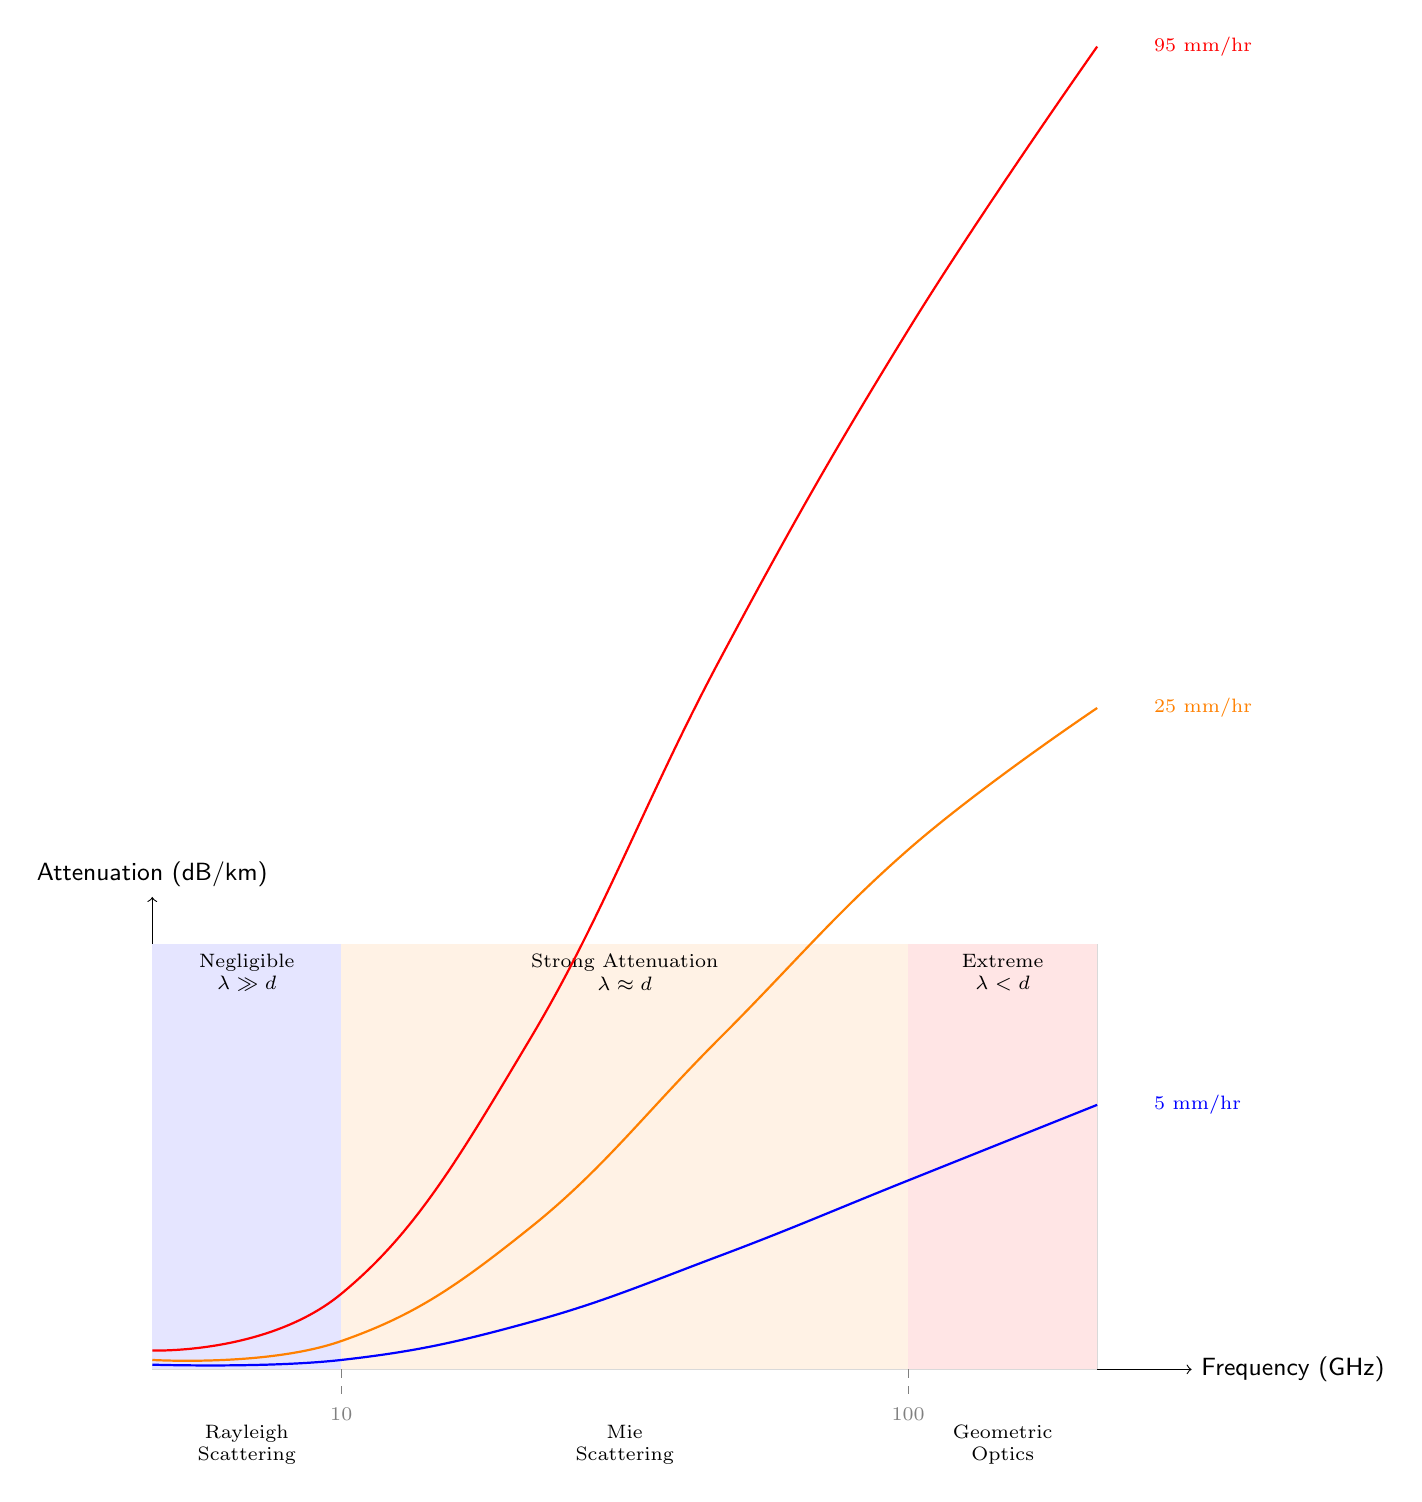
\begin{tikzpicture}[scale=1.2]
% Axes
\draw[->] (0,0) -- (11,0) node[right] {\sffamily\small Frequency (GHz)};
\draw[->] (0,0) -- (0,5) node[above] {\sffamily\small Attenuation (dB/km)};

% Grid
\draw[very thin,gray!30] (0,0) grid[step=1] (10,4.5);

% Frequency regions
\fill[blue!10] (0,0) rectangle (2,4.5);
\fill[orange!10] (2,0) rectangle (8,4.5);
\fill[red!10] (8,0) rectangle (10,4.5);

% Region labels
\node[align=center,font=\scriptsize] at (1,4.2) {Negligible\\$\lambda \gg d$};
\node[align=center,font=\scriptsize] at (5,4.2) {Strong Attenuation\\$\lambda \approx d$};
\node[align=center,font=\scriptsize] at (9,4.2) {Extreme\\$\lambda < d$};

% Attenuation curves for different rain rates
\draw[thick,blue] plot[smooth,tension=0.7] coordinates {(0,0.05) (2,0.1) (4,0.5) (6,1.2) (8,2.0) (10,2.8)};
\draw[thick,orange] plot[smooth,tension=0.7] coordinates {(0,0.1) (2,0.3) (4,1.5) (6,3.5) (8,5.5) (10,7.0)};
\draw[thick,red] plot[smooth,tension=0.7] coordinates {(0,0.2) (2,0.8) (4,3.5) (6,7.5) (8,11) (10,14)};

% Legend
\node[right,font=\scriptsize,blue] at (10.5,2.8) {5 mm/hr};
\node[right,font=\scriptsize,orange] at (10.5,7.0) {25 mm/hr};
\node[right,font=\scriptsize,red] at (10.5,14) {95 mm/hr};

% Frequency markers
\draw[dashed,gray] (2,0) -- (2,-0.3) node[below,font=\scriptsize] {10};
\draw[dashed,gray] (8,0) -- (8,-0.3) node[below,font=\scriptsize] {100};

% Wavelength annotations
\node[font=\scriptsize,align=center] at (1,-0.8) {Rayleigh\\Scattering};
\node[font=\scriptsize,align=center] at (5,-0.8) {Mie\\Scattering};
\node[font=\scriptsize,align=center] at (9,-0.8) {Geometric\\Optics};
\end{tikzpicture}
\end{center}

\begin{itemize}
\item \textbf{Below 10~GHz}: Rain effects negligible. Wavelength ($\lambda > 3$~cm) is much larger than typical raindrop diameter (1--5~mm). Rayleigh scattering regime.

\item \textbf{10--100~GHz}: Strong attenuation. Wavelength comparable to raindrop size, maximizing interaction cross-section. Mie scattering regime dominates.

\item \textbf{Above 100~GHz}: Extreme attenuation. Short wavelengths ($\lambda < 3$~mm) are heavily absorbed and scattered. Terahertz communications become impractical in rain.
\end{itemize}

\subsection{ITU-R Rain Attenuation Model}

The International Telecommunication Union provides standardized methods for predicting rain attenuation through recommendations \textbf{ITU-R P.838} (specific attenuation coefficients) and \textbf{ITU-R P.618} (propagation data and methods).

\subsubsection{Specific Attenuation Formula}

The specific attenuation per kilometer of path is given by:
\begin{equation}
\gamma_R = k \cdot R^\alpha \quad \text{(dB/km)}
\label{eq:rain-specific-atten}
\end{equation}
where:
\begin{itemize}
\item $\gamma_R$ = specific attenuation (dB/km)
\item $R$ = rainfall rate (mm/hr)
\item $k, \alpha$ = frequency- and polarization-dependent regression coefficients
\end{itemize}

The total path attenuation is:
\begin{equation}
A_{\text{rain}} = \gamma_R \cdot d_{\text{eff}} \quad \text{(dB)}
\label{eq:total-rain-atten}
\end{equation}
where $d_{\text{eff}}$ is the effective path length through rain (km).

\subsubsection{ITU Coefficients by Frequency}

Table~\ref{tab:itu-rain-coeffs} provides selected ITU-R P.838 coefficients for horizontal polarization.

\begin{table}[h!]
\centering
\caption{ITU-R rain attenuation coefficients (horizontal polarization)}
\label{tab:itu-rain-coeffs}
\begin{tabular}{@{}lccr@{}}
\toprule
Frequency & $k$ & $\alpha$ & $\gamma_R$ @ 25~mm/hr \\
\midrule
1~GHz & 0.0000387 & 0.912 & 0.0005~dB/km \\
4~GHz (C-band) & 0.00065 & 1.121 & 0.025~dB/km \\
10~GHz (X-band) & 0.0101 & 1.276 & 0.50~dB/km \\
12~GHz (Ku-band) & 0.0188 & 1.310 & 1.02~dB/km \\
20~GHz (Ka-band) & 0.0751 & 1.099 & 3.26~dB/km \\
30~GHz & 0.187 & 1.021 & 7.14~dB/km \\
40~GHz (V-band) & 0.350 & 0.939 & 12.2~dB/km \\
50~GHz & 0.536 & 0.873 & 16.8~dB/km \\
60~GHz & 0.707 & 0.826 & 20.3~dB/km \\
80~GHz (W-band) & 0.999 & 0.784 & 26.4~dB/km \\
100~GHz & 1.187 & 0.751 & 29.8~dB/km \\
\bottomrule
\end{tabular}
\end{table}

\begin{calloutbox}{Polarization Effects}
Vertical polarization typically experiences 10--20\% more attenuation than horizontal polarization due to the oblate (flattened) shape of raindrops. For critical link budget calculations, use polarization-specific coefficients from ITU-R P.838 tables.
\end{calloutbox}

\subsection{Rain Rate Classifications}

The ITU divides the world into \textbf{rain climate zones} based on statistical rainfall data. System designers use these zones to determine appropriate link margins.

\begin{table}[h!]
\centering
\caption{ITU-R rain climate zones}
\label{tab:itu-rain-zones}
\begin{tabular}{@{}llrl@{}}
\toprule
Zone & Climate & $R_{0.01}$ (mm/hr) & Example Locations \\
\midrule
A & Polar & 8 & Arctic, Antarctic \\
B & Temperate & 12 & Northern Europe, Canada \\
C & Subtropical & 22 & Southern US, Mediterranean \\
D & Moderate tropical & 32 & Southeast Asia, India \\
E & Equatorial & 42 & Central Africa, Indonesia \\
F & Tropical maritime & 53 & Amazon, Congo Basin \\
G & Monsoon & 63 & Bangladesh, Myanmar \\
H & Intense tropical & 95 & Extreme thunderstorms \\
\bottomrule
\end{tabular}
\end{table}

where $R_{0.01}$ is the rainfall rate exceeded for 0.01\% of an average year (approximately 53~minutes annually). This corresponds to the \textbf{99.99\% link availability} design criterion.

\begin{center}
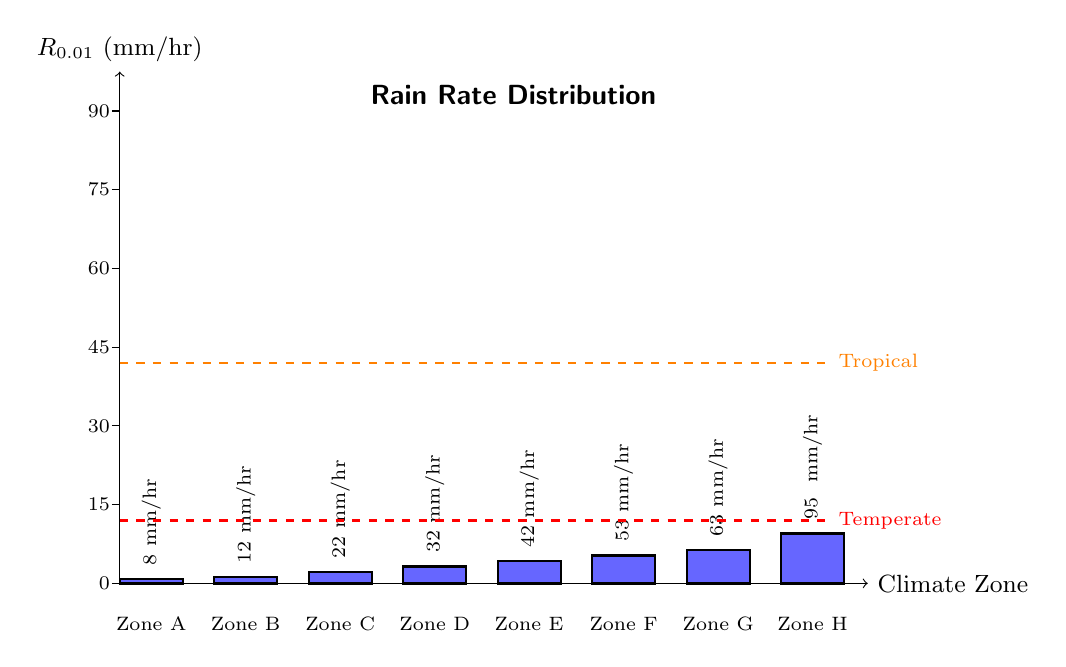
\begin{tikzpicture}[scale=1.0]
% Title
\node[font=\sffamily\bfseries] at (5,6.2) {Rain Rate Distribution};

% Bar chart for rain zones
\foreach \x/\height/\label/\rate in {
  0/0.8/A/8,
  1.2/1.2/B/12,
  2.4/2.2/C/22,
  3.6/3.2/D/32,
  4.8/4.2/E/42,
  6.0/5.3/F/53,
  7.2/6.3/G/63,
  8.4/9.5/H/95
} {
  \fill[blue!60] (\x,0) rectangle +(0.8,\height/15);
  \draw[thick] (\x,0) rectangle +(0.8,\height/15);
  \node[below,font=\scriptsize] at (\x+0.4,-0.3) {Zone \label};
  \node[above,font=\scriptsize,rotate=90,anchor=west] at (\x+0.4,\height/15+0.05) {\rate~mm/hr};
}

% Y-axis
\draw[->] (0,0) -- (0,6.5) node[above,font=\small] {$R_{0.01}$ (mm/hr)};
\foreach \y in {0,15,30,45,60,75,90} {
  \draw (-0.1,\y/15) -- (0,\y/15) node[left,font=\scriptsize] {\y};
}

% X-axis
\draw[->] (0,0) -- (9.5,0) node[right,font=\small] {Climate Zone};

% Threshold lines
\draw[dashed,red,thick] (0,0.8) -- (9,0.8) node[right,font=\scriptsize] {Temperate};
\draw[dashed,orange,thick] (0,2.8) -- (9,2.8) node[right,font=\scriptsize] {Tropical};

\end{tikzpicture}
\end{center}

\textbf{Design Guidelines:}
\begin{itemize}
\item \textbf{Temperate regions}: Design for $R = 12$~mm/hr (Zone B)
\item \textbf{Tropical regions}: Design for $R = 42$--63~mm/hr (Zones E--G)
\item \textbf{Critical links}: Add margin for extreme events (Zone H)
\end{itemize}

\section{Worked Examples}

\subsection{Example 1: Ku-Band Satellite Downlink}

\textbf{Scenario:} Geostationary Earth orbit (GEO) satellite downlink to home receiver in temperate climate.

\vspace{6pt}
\textbf{Given Parameters:}
\begin{itemize}
\item Frequency: $f = 12$~GHz (Ku-band)
\item Elevation angle: $\theta = 30°$
\item Effective rain path length: $d_{\text{eff}} \approx 6$~km
\item Rain rate (Zone B, 0.01\% time): $R = 12$~mm/hr
\item ITU coefficients: $k = 0.0188$, $\alpha = 1.310$
\end{itemize}

\vspace{6pt}
\textbf{Step 1: Calculate Specific Attenuation}

Using Equation~\ref{eq:rain-specific-atten}:
\begin{equation}
\gamma_R = k \cdot R^\alpha = 0.0188 \times 12^{1.310} = 0.50~\text{dB/km}
\end{equation}

\textbf{Step 2: Calculate Total Path Attenuation}

Using Equation~\ref{eq:total-rain-atten}:
\begin{equation}
A_{\text{rain}} = \gamma_R \times d_{\text{eff}} = 0.50 \times 6 = 3.0~\text{dB}
\end{equation}

\textbf{Result:} A \textbf{3~dB rain fade margin} is required for 99.99\% link availability in temperate climates.

\vspace{10pt}
\textbf{Extreme Storm Scenario (Zone H):}

For an extreme thunderstorm with $R = 95$~mm/hr:
\begin{equation}
\gamma_R = 0.0188 \times 95^{1.310} = 6.3~\text{dB/km}
\end{equation}
\begin{equation}
A_{\text{rain}} = 6.3 \times 6 = 38~\text{dB}
\end{equation}

\begin{warningbox}
A 38~dB fade \textbf{exceeds typical Ku-band link margins} (10--15~dB), resulting in complete signal outage. Such extreme events occur rarely but must be considered for critical applications.
\end{warningbox}

\subsection{Example 2: Ka-Band Satellite Link}

\textbf{Scenario:} Same GEO satellite geometry as Example 1, but using Ka-band frequency.

\vspace{6pt}
\textbf{Given Parameters:}
\begin{itemize}
\item Frequency: $f = 20$~GHz (Ka-band)
\item Path length: $d_{\text{eff}} = 6$~km
\item ITU coefficients: $k = 0.0751$, $\alpha = 1.099$
\end{itemize}

\vspace{6pt}
\textbf{Case 1: Temperate Climate ($R = 12$~mm/hr)}

\begin{equation}
\gamma_R = 0.0751 \times 12^{1.099} = 1.16~\text{dB/km}
\end{equation}
\begin{equation}
A_{\text{rain}} = 1.16 \times 6 = 7.0~\text{dB}
\end{equation}

\textbf{Case 2: Tropical Climate ($R = 42$~mm/hr)}

\begin{equation}
\gamma_R = 0.0751 \times 42^{1.099} = 4.4~\text{dB/km}
\end{equation}
\begin{equation}
A_{\text{rain}} = 4.4 \times 6 = 26~\text{dB}
\end{equation}

\begin{keyconcept}
\textbf{Frequency Penalty:} Ka-band (20~GHz) suffers approximately \textbf{2.3$\times$ more rain fade} than Ku-band (12~GHz) for the same rainfall rate and path geometry. This frequency-dependent penalty must be carefully considered when selecting communication bands.
\end{keyconcept}

\textbf{Mitigation Strategies:}
\begin{itemize}
\item \textbf{Adaptive Coding/Modulation (ACM)}: Dynamically reduce data rate during rain
\item \textbf{Site diversity}: Multiple ground stations separated by 5--20~km
\item \textbf{Increased link margin}: Add 10--15~dB for tropical deployments
\item \textbf{Uplink power control}: Boost transmit power during fade events
\end{itemize}

\subsection{Example 3: 5G mmWave Urban Link}

\textbf{Scenario:} 5G base station to user equipment in urban environment.

\vspace{6pt}
\textbf{Given Parameters:}
\begin{itemize}
\item Frequency: $f = 28$~GHz (5G mmWave)
\item Path length: $d = 200$~m $= 0.2$~km
\item ITU coefficients: $k = 0.187$, $\alpha = 1.021$
\end{itemize}

\vspace{6pt}
\textbf{Light Rain ($R = 5$~mm/hr):}
\begin{equation}
\gamma_R = 0.187 \times 5^{1.021} = 0.98~\text{dB/km}
\end{equation}
\begin{equation}
A_{\text{rain}} = 0.98 \times 0.2 = 0.2~\text{dB}
\end{equation}

\textbf{Heavy Rain ($R = 25$~mm/hr):}
\begin{equation}
\gamma_R = 0.187 \times 25^{1.021} = 5.2~\text{dB/km}
\end{equation}
\begin{equation}
A_{\text{rain}} = 5.2 \times 0.2 = 1.0~\text{dB}
\end{equation}

\begin{calloutbox}{5G mmWave Rain Tolerance}
\textbf{Short-range 5G links ($<$ 500~m) are relatively rain-tolerant.} The high specific attenuation at 28~GHz is offset by short path lengths. A 1~dB fade in heavy rain can typically be absorbed by existing link margins.

However, for longer backhaul links or satellite connections, mmWave frequencies require significant additional margin or mitigation techniques.
\end{calloutbox}

\section{Fog and Cloud Attenuation}

\subsection{Physical Characteristics}

Fog consists of \textbf{suspended water droplets} with typical diameters of 10--100~$\mu$m, significantly smaller than raindrops (1--5~mm). The primary attenuation mechanism is \textbf{absorption} rather than scattering, since droplet size $d \ll \lambda$ for most microwave and millimeter-wave frequencies (Rayleigh regime).

\subsection{Fog Attenuation Model}

The specific attenuation due to fog is given by:
\begin{equation}
\gamma_{\text{fog}} = K_l \cdot M \quad \text{(dB/km)}
\label{eq:fog-atten}
\end{equation}
where:
\begin{itemize}
\item $M$ = liquid water content (g/m$^3$)
\item $K_l$ = frequency-dependent specific attenuation coefficient (dB$\cdot$km$^{-1}$/(g/m$^3$))
\end{itemize}

\textbf{Typical fog conditions:}
\begin{itemize}
\item Light fog: $M = 0.05$~g/m$^3$ (visibility $\approx$ 1~km)
\item Moderate fog: $M = 0.2$~g/m$^3$ (visibility $\approx$ 300~m)
\item Dense fog: $M = 0.5$~g/m$^3$ (visibility $< 100$~m)
\end{itemize}

\subsection{Fog Attenuation Coefficients}

Table~\ref{tab:fog-coeffs} provides frequency-dependent fog attenuation coefficients.

\begin{table}[h!]
\centering
\caption{Fog attenuation coefficients and representative values}
\label{tab:fog-coeffs}
\begin{tabular}{@{}crr@{}}
\toprule
Frequency & $K_l$ (dB/km per g/m$^3$) & $\gamma$ (dense fog, $M = 0.5$~g/m$^3$) \\
\midrule
10~GHz & 0.01 & 0.005~dB/km \\
20~GHz & 0.07 & 0.035~dB/km \\
30~GHz & 0.20 & 0.10~dB/km \\
60~GHz & 1.0 & 0.50~dB/km \\
100~GHz & 2.5 & 1.25~dB/km \\
300~GHz & 15 & 7.5~dB/km \\
\bottomrule
\end{tabular}
\end{table}

\begin{keyconcept}
\textbf{Fog vs Rain:} Below 30~GHz, fog attenuation is \textbf{negligible compared to rain}. However, at terahertz frequencies ($>$ 100~GHz), fog becomes a significant impairment, particularly for short-range THz communication systems.
\end{keyconcept}

\subsection{Rain vs Fog: Comparative Analysis}

\subsubsection{Microwave/mmWave Regime (30~GHz, 1~km path)}

\begin{table}[h!]
\centering
\caption{Weather attenuation comparison at 30~GHz}
\label{tab:rain-fog-30ghz}
\begin{tabular}{@{}lr@{}}
\toprule
Weather Condition & Total Attenuation \\
\midrule
Clear air & $\sim$0.1~dB \\
Dense fog ($M = 0.5$~g/m$^3$) & 0.10~dB \\
Light rain ($R = 5$~mm/hr) & 3.7~dB \\
Moderate rain ($R = 12$~mm/hr) & 7.1~dB \\
Heavy rain ($R = 25$~mm/hr) & 12.5~dB \\
\bottomrule
\end{tabular}
\end{table}

\textbf{Conclusion:} At microwave and millimeter-wave frequencies, \textbf{rain dominates} weather-induced attenuation. Fog is negligible by comparison.

\subsubsection{Terahertz Regime (300~GHz, 100~m path)}

\begin{table}[h!]
\centering
\caption{Weather attenuation comparison at 300~GHz (THz)}
\label{tab:rain-fog-300ghz}
\begin{tabular}{@{}lr@{}}
\toprule
Weather Condition & Total Attenuation \\
\midrule
Clear air (water vapor) & $\sim$5~dB \\
Dense fog ($M = 0.5$~g/m$^3$) & 0.75~dB \\
Light rain ($R = 5$~mm/hr) & $>$ 300~dB (complete blockage) \\
\bottomrule
\end{tabular}
\end{table}

\begin{center}
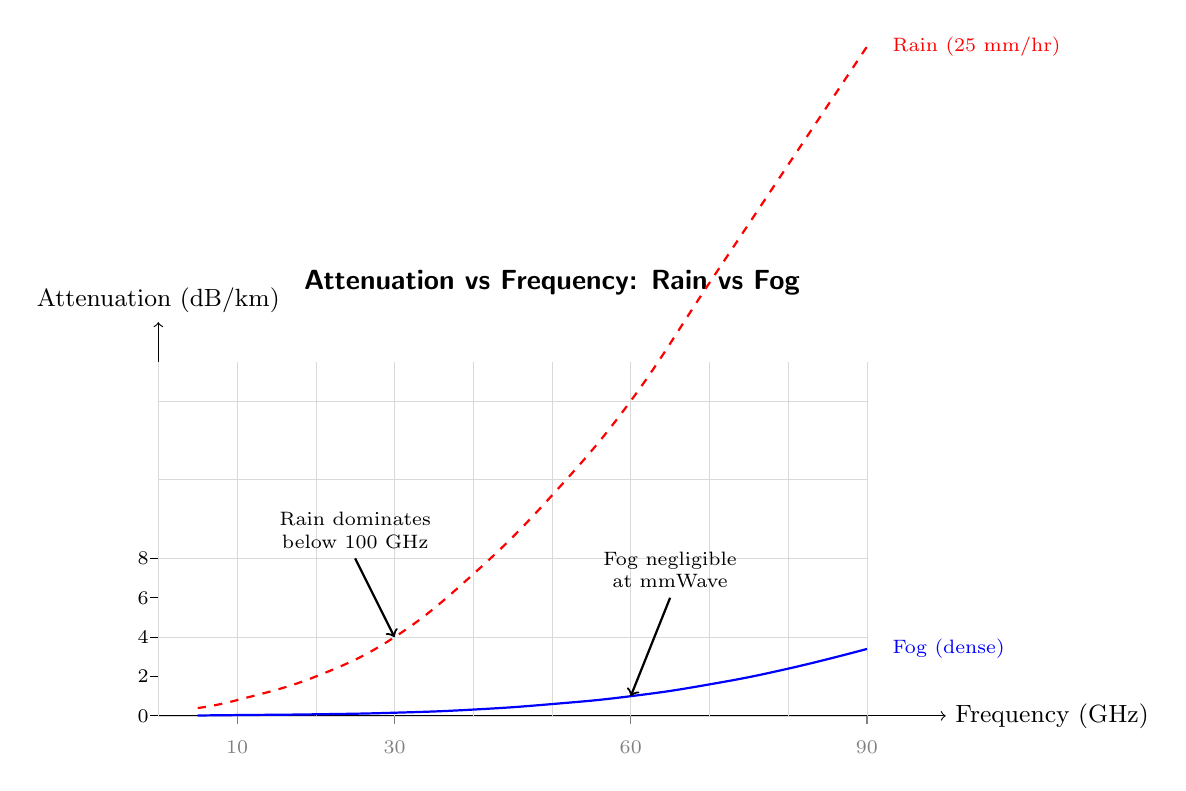
\begin{tikzpicture}[scale=1.0]
% Title
\node[font=\sffamily\bfseries] at (5,5.5) {Attenuation vs Frequency: Rain vs Fog};

% Axes
\draw[->] (0,0) -- (10,0) node[right,font=\small] {Frequency (GHz)};
\draw[->] (0,0) -- (0,5) node[above,font=\small] {Attenuation (dB/km)};

% Grid
\draw[very thin,gray!30] (0,0) grid[step=1] (9,4.5);

% Rain curves (25 mm/hr)
\draw[thick,red,dashed] plot[smooth,tension=0.7] coordinates {
  (0.5,0.1) (1,0.2) (2,0.5) (3,1.0) (4,1.8) (5,2.8) (6,4.0) (7,5.5) (8,7.0) (9,8.5)
};
\node[right,font=\scriptsize,red] at (9.2,8.5) {Rain (25~mm/hr)};

% Fog curve (dense fog, 0.5 g/m³)
\draw[thick,blue] plot[smooth,tension=0.8] coordinates {
  (0.5,0.005) (1,0.01) (2,0.02) (3,0.04) (4,0.08) (5,0.15) (6,0.25) (7,0.40) (8,0.60) (9,0.85)
};
\node[right,font=\scriptsize,blue] at (9.2,0.85) {Fog (dense)};

% Frequency markers
\foreach \x/\label in {1/10, 3/30, 6/60, 9/90} {
  \draw[dashed,gray] (\x,0) -- (\x,-0.2) node[below,font=\scriptsize] {\label};
}

% Attenuation scale
\foreach \y/\label in {0/0, 1/2, 2/4, 3/6, 4/8} {
  \draw (-0.1,\y*0.5) -- (0,\y*0.5) node[left,font=\scriptsize] {\label};
}

% Annotation
\draw[<-,thick] (3,1.0) -- (2.5,2) node[above,font=\scriptsize,align=center] {Rain dominates\\below 100~GHz};
\draw[<-,thick] (6,0.25) -- (6.5,1.5) node[above,font=\scriptsize,align=center] {Fog negligible\\at mmWave};

\end{tikzpicture}
\end{center}

\textbf{Design Implication:} For frequencies below 100~GHz, link budgets should primarily account for rain attenuation. Fog can generally be ignored. At THz frequencies, both rain and fog must be considered, with rain causing catastrophic attenuation.

\section{Snow and Ice Effects}

\subsection{Dry Snow Attenuation}

Dry snow consists of ice crystals and air pockets with very low dielectric loss. The specific attenuation is approximated by:
\begin{equation}
\gamma_{\text{dry snow}} \approx 0.0005 \times f^2 \times S \quad \text{(dB/km)}
\label{eq:dry-snow}
\end{equation}
where $f$ is frequency (GHz) and $S$ is snowfall rate (mm/hr liquid water equivalent).

\textbf{Example:} At 20~GHz with $S = 10$~mm/hr:
\begin{equation}
\gamma_{\text{dry snow}} = 0.0005 \times 20^2 \times 10 = 0.2~\text{dB/km}
\end{equation}

This is \textbf{negligible} compared to rain at the same frequency.

\subsection{Wet Snow and Ice}

\begin{itemize}
\item \textbf{Wet snow} (melting): Attenuation comparable to rain due to liquid water content
\item \textbf{Ice crystals} (cirrus clouds): Minimal attenuation ($< 0.1$~dB even at 100~GHz)
\item \textbf{Hailstones}: Lower attenuation than rain of equivalent water content, since ice has lower loss tangent ($\tan\delta_{\text{ice}} \ll \tan\delta_{\text{water}}$)
\end{itemize}

\begin{calloutbox}{Practical Implications}
\textbf{Snow is far less problematic than rain for RF links.} Dry snow can be essentially ignored in link budget calculations below 100~GHz. The primary concern with hail is not attenuation but \textbf{depolarization}---tumbling hailstones scatter energy to the cross-polarization, degrading dual-polarization systems.
\end{calloutbox}

\section{Frequency Band Sensitivity}

Different frequency bands exhibit vastly different susceptibility to rain attenuation, influencing their suitability for various applications.

\begin{table}[h!]
\centering
\caption{Rain sensitivity by frequency band}
\label{tab:band-sensitivity}
\begin{tabular}{@{}llll@{}}
\toprule
Band & Frequency & Primary Use & Rain Sensitivity @ 25~mm/hr \\
\midrule
C-band & 4--8~GHz & Satellite TV, radar & \textbf{Low} (0.05~dB/km) \\
X-band & 8--12~GHz & Military, radar & \textbf{Moderate} (0.5~dB/km) \\
Ku-band & 12--18~GHz & Satellite TV/broadband & \textbf{Moderate-High} (1--2~dB/km) \\
Ka-band & 26.5--40~GHz & Satellite, 5G backhaul & \textbf{High} (3--12~dB/km) \\
V-band & 40--75~GHz & Next-gen satellite & \textbf{Very High} (12--20~dB/km) \\
W-band & 75--110~GHz & Automotive radar & \textbf{Extreme} (20--30~dB/km) \\
\bottomrule
\end{tabular}
\end{table}

\textbf{C-band Advantage:} Widely deployed in tropical regions due to excellent rain tolerance. Lower bandwidth but highly reliable.

\textbf{Ka-band Challenge:} Offers high data rates and bandwidth, but requires adaptive coding/modulation (ACM) and large link margins (10--15~dB) to maintain availability.

\section{Mitigation Techniques}

Engineers employ several strategies to maintain link availability despite weather-induced attenuation.

\subsection{Static Link Margin}

The simplest approach is to \textbf{add extra power margin} to the link budget:

\begin{itemize}
\item Temperate climate, Ku-band: +3--5~dB
\item Tropical climate, Ka-band: +8--15~dB
\item mmWave terrestrial ($< 1$~km): +2--3~dB
\end{itemize}

\textbf{Trade-off:} Requires higher transmit power or larger antennas, increasing cost and complexity.

\subsection{Adaptive Coding and Modulation (ACM)}

ACM systems \textbf{dynamically adjust modulation order and coding rate} based on real-time link quality:

\begin{center}
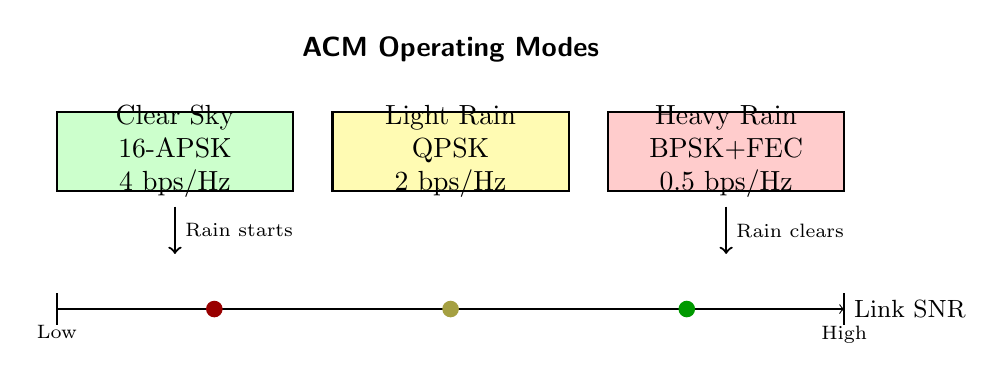
\begin{tikzpicture}[scale=1.0]
% Title
\node[font=\sffamily\bfseries] at (5,4.8) {ACM Operating Modes};

% States
\draw[fill=green!20,thick] (0,3) rectangle (3,4) node[pos=0.5,align=center] {Clear Sky\\16-APSK\\4 bps/Hz};
\draw[fill=yellow!30,thick] (3.5,3) rectangle (6.5,4) node[pos=0.5,align=center] {Light Rain\\QPSK\\2 bps/Hz};
\draw[fill=red!20,thick] (7,3) rectangle (10,4) node[pos=0.5,align=center] {Heavy Rain\\BPSK+FEC\\0.5 bps/Hz};

% Arrows showing transitions
\draw[->,thick] (1.5,2.8) -- (1.5,2.2) node[midway,right,font=\scriptsize] {Rain starts};
\draw[->,thick] (8.5,2.8) -- (8.5,2.2) node[midway,right,font=\scriptsize] {Rain clears};

% SNR axis
\draw[->] (0,1.5) -- (10,1.5) node[right,font=\small] {Link SNR};
\draw[thick] (0,1.3) -- (0,1.7) node[below=8pt,font=\scriptsize] {Low};
\draw[thick] (10,1.3) -- (10,1.7) node[below=8pt,font=\scriptsize] {High};

% Operating points
\fill[green!60!black] (8,1.5) circle (3pt);
\fill[yellow!60!black] (5,1.5) circle (3pt);
\fill[red!60!black] (2,1.5) circle (3pt);

\end{tikzpicture}
\end{center}

\textbf{Result:} Graceful degradation---system maintains connectivity at reduced data rate rather than complete outage.

\textbf{Applications:} DVB-S2 (satellite TV), 5G NR, VSAT modems.

\subsection{Site Diversity}

Multiple ground stations separated by 5--20~km exploit the \textbf{localized nature of rain cells} (typically 5--10~km diameter):

\begin{equation}
P_{\text{both fade}} = P_{\text{site 1}} \times P_{\text{site 2}} \times \rho
\end{equation}
where $\rho < 1$ is the spatial correlation factor.

\textbf{Diversity gain:} 5--10~dB improvement in link availability.

\textbf{Example:} Commercial satellite gateways deploy 2--3 geographically separated sites to achieve 99.99\% uptime.

\subsection{Uplink Power Control (UPC)}

UPC systems \textbf{increase transmit power during rain} to compensate for attenuation:

\begin{enumerate}
\item Monitor satellite beacon signal strength
\item Detect fade depth in real-time
\item Boost uplink power (typically up to 10~dB)
\item Avoid saturating satellite transponder
\end{enumerate}

\textbf{Limitation:} Power amplifier headroom is finite. Cannot compensate for extreme fades ($> 15$~dB).

\subsection{Orbit Selection}

Low Earth Orbit (LEO) satellites offer \textbf{inherently shorter rain paths}:

\begin{itemize}
\item \textbf{GEO} (36,000~km altitude): Rain path $\approx 6$~km at 30° elevation
\item \textbf{LEO} (550~km altitude): Rain path $\approx 2$~km at 30° elevation
\end{itemize}

\textbf{Result:} LEO systems experience approximately \textbf{3$\times$ less rain attenuation} than GEO for the same frequency and rain rate. This is a key advantage of Starlink and OneWeb constellations.

\section{Depolarization Effects}

Beyond simple attenuation, rain also causes \textbf{cross-polarization interference} due to the oblate (flattened) shape of raindrops.

\subsection{Physical Mechanism}

Raindrops are not spherical---they flatten into oblate spheroids as they fall. This asymmetry causes:
\begin{itemize}
\item Different phase shifts for horizontal and vertical polarization components
\item Coupling of energy from the co-polarized channel to the cross-polarized channel
\end{itemize}

\subsection{Cross-Polarization Discrimination (XPD)}

The rain-induced XPD degradation is modeled by:
\begin{equation}
\text{XPD}_{\text{rain}} = U - V \log_{10}(A_{\text{rain}}) \quad \text{(dB)}
\label{eq:xpd-rain}
\end{equation}
where:
\begin{itemize}
\item $U, V$ = frequency-dependent constants (typically $U = 30$--40~dB, $V = 12$--20~dB)
\item $A_{\text{rain}}$ = co-polarization attenuation (dB)
\end{itemize}

\textbf{Example:} If rain causes $A_{\text{rain}} = 10$~dB attenuation:
\begin{equation}
\text{XPD}_{\text{rain}} = 30 - 12 \times \log_{10}(10) = 30 - 12 = 18~\text{dB}
\end{equation}

The XPD degrades from 30~dB (clear sky) to 18~dB (rain), reducing the isolation between orthogonal polarization channels.

\textbf{Impact:} Degrades dual-polarization systems that use V/H reuse to double capacity (e.g., satellite transponders, point-to-point microwave links).

\section{Applications}

\subsection{Satellite Communications}

Weather effects are most critical for satellite links operating above 10~GHz:

\begin{itemize}
\item \textbf{Direct-to-Home (DTH) TV}: Ku-band systems require 3--8~dB rain margin depending on climate zone. Service outages during extreme storms are accepted.

\item \textbf{VSAT Networks}: Ka-band systems use ACM to maintain connectivity. Typical availability: 99.5--99.9\% depending on required data rate.

\item \textbf{LEO Broadband}: Starlink and OneWeb operate at Ka/Ku bands but benefit from shorter rain paths. Beam switching between satellites provides diversity.
\end{itemize}

\subsection{5G Millimeter-Wave}

5G systems at 28/39/60~GHz face rain challenges primarily for backhaul links:

\begin{itemize}
\item \textbf{Access links} ($< 500$~m): Rain fade typically $< 2$~dB, absorbed by link margin
\item \textbf{Backhaul links} (1--5~km): Require 5--10~dB additional margin or diversity
\item \textbf{Fixed wireless access (FWA)}: ACM and beam steering mitigate rain effects
\end{itemize}

\subsection{Point-to-Point Microwave}

Terrestrial microwave links (6--80~GHz) for cellular backhaul and enterprise connectivity:

\begin{itemize}
\item \textbf{Licensed bands} (18/23/38~GHz): Careful link budget planning with rain margin
\item \textbf{60~GHz unlicensed}: Limited to $< 1$~km due to oxygen absorption + rain
\item \textbf{Diversity schemes}: Hot standby links at lower frequency or spatial diversity
\end{itemize}

\subsection{Radar and Remote Sensing}

\begin{itemize}
\item \textbf{Weather radar}: Exploits rain backscatter (10~GHz X-band, 5~GHz C-band)
\item \textbf{Cloud radar}: Uses Ka/W-band (35/94~GHz) to detect clouds and precipitation
\item \textbf{Radiometers}: Measure sky brightness temperature to infer rain rate and liquid water content
\end{itemize}

\section{Summary}

Weather-induced attenuation is a critical propagation impairment that increases dramatically with frequency and precipitation rate.

\subsection{Key Design Parameters}

\begin{table}[h!]
\centering
\caption{Rain attenuation summary for 6~km satellite path (30° elevation)}
\label{tab:summary-rain-atten}
\begin{tabular}{@{}lcrr@{}}
\toprule
Band & Frequency & Temperate (12~mm/hr) & Tropical (42~mm/hr) \\
\midrule
C-band & 4~GHz & 0.15~dB & 0.7~dB \\
X-band & 10~GHz & 0.5~dB & 2.5~dB \\
\textbf{Ku-band} & \textbf{12~GHz} & \textbf{3~dB} & \textbf{9~dB} \\
\textbf{Ka-band} & \textbf{20~GHz} & \textbf{7~dB} & \textbf{22~dB} \\
V-band & 40~GHz & 22~dB & 60~dB \\
\bottomrule
\end{tabular}
\end{table}

\subsection{Design Guidelines}

\begin{enumerate}
\item \textbf{Frequency Selection:}
  \begin{itemize}
  \item C-band: Robust in all climates, bandwidth-limited
  \item Ku-band: Good balance for temperate regions
  \item Ka-band: High capacity, requires mitigation
  \item mmWave: Only for short terrestrial or inter-satellite links
  \end{itemize}

\item \textbf{Link Margin Allocation:}
  \begin{itemize}
  \item Temperate: 3--8~dB (frequency-dependent)
  \item Tropical: 10--25~dB for Ka-band and above
  \item Consider 99.9\% or 99.99\% availability requirement
  \end{itemize}

\item \textbf{Mitigation Strategy:}
  \begin{itemize}
  \item Static margin: Simplest, highest cost
  \item ACM: Graceful degradation, widely deployed
  \item Site diversity: Excellent for fixed gateways
  \item LEO orbit: Inherently rain-tolerant
  \end{itemize}
\end{enumerate}

\begin{keyconcept}
\textbf{The rain fade dilemma:} Higher frequencies offer greater bandwidth and smaller antennas, but suffer exponentially more rain attenuation. System design requires careful trade-offs between capacity, cost, and availability based on climate zone and application requirements.
\end{keyconcept}

\section{Further Reading}

\begin{itemize}
\item Chapter~\ref{ch:fspl}: Free-Space Path Loss---baseline propagation model
\item Chapter~\ref{ch:atmospheric}: Atmospheric Effects---clear-air absorption
\item Chapter~\ref{ch:multipath}: Multipath Propagation---Rayleigh and Rician fading
\item Chapter~\ref{ch:snr}: Signal-to-Noise Ratio---link quality metrics
\item Chapter~\ref{ch:link-budget}: Link Budget Analysis---system-level design
\item ITU-R Recommendations P.838, P.618, P.676---authoritative references for rain and atmospheric models
\end{itemize}
